\chapter{Prezentacja elementów projektu:}
\label{cha:elementyPracy}

% ------------------------------------------------------------------------


% ------------------------------------------------------------------------
\section{Prezentacja warstwy użytkowej}

Główne okno aplikacji.

\begin{figure}[H]
	\centering
	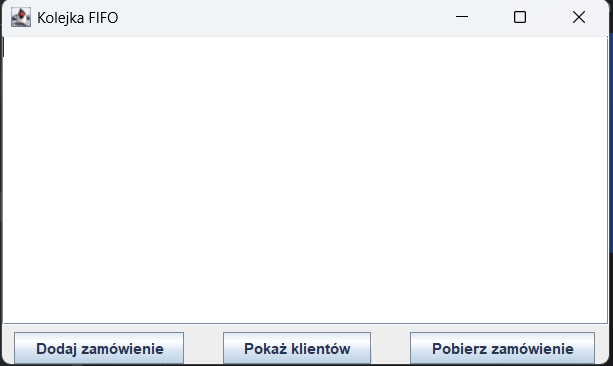
\includegraphics[width=0.7\linewidth]{figures/screenshot001}
	\caption{Okno główne}
	\label{fig:screenshot001}
\end{figure}
 
% ------------------------------------------------------------------------
Dodawanie zamówień:

Aby dodać zamówienie należy, nacisnąć przycisk "Dodaj zamówienie". W następnym kroku podajemy
imię i nazwisko


\begin{figure}[H]
	\centering
	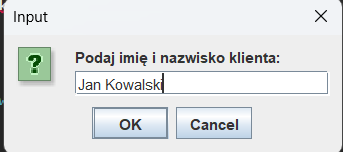
\includegraphics[width=0.7\linewidth]{figures/screenshot002}
	\caption{Podawanie Imiona i nazwiska klienta}
	\label{fig:screenshot002}
\end{figure}
Gdy Klikniemy Ok, program poprosi o wpisanie adresu e-mail.

\begin{figure}[H]
	\centering
	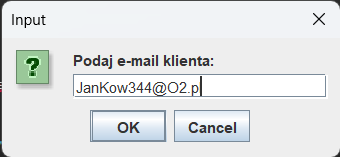
\includegraphics[width=0.7\linewidth]{figures/screenshot003}
	\caption{Wpisywanie Adresu Email}
	\label{fig:screenshot003}
\end{figure}
Po wpisaniu e-maila i wciśnięciu ok, program nas poprosi o wpisanie ilości przedmiotów jaki dany
klient kupił.
\begin{figure}[H]
	\centering
	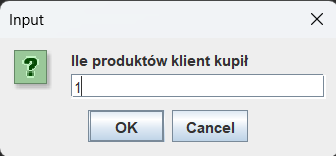
\includegraphics[width=0.7\linewidth]{figures/screenshot004}
	\caption{Podawanie ilości przedmiotów}
	\label{fig:screenshot004}
\end{figure}
Następnie program poprosi o Nazwę produktu, oraz o jego cenę.
\begin{figure}[H]
	\centering
	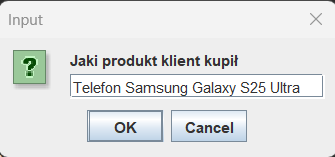
\includegraphics[width=0.7\linewidth]{figures/screenshot005}
	\caption{Podawanie nazwy produktu}
	\label{fig:screenshot005}
\end{figure}
\begin{figure}[H]
	\centering
	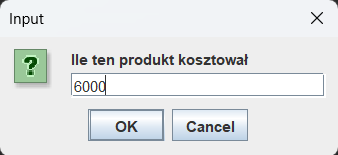
\includegraphics[width=0.7\linewidth]{figures/screenshot006}
	\caption{Podawanie ceny produktu}
	\label{fig:screenshot006}
\end{figure}
Po zakończeniu wszystkich powyższych kroków, program wypisze, dane zamówienia.
\begin{figure}[H]
	\centering
	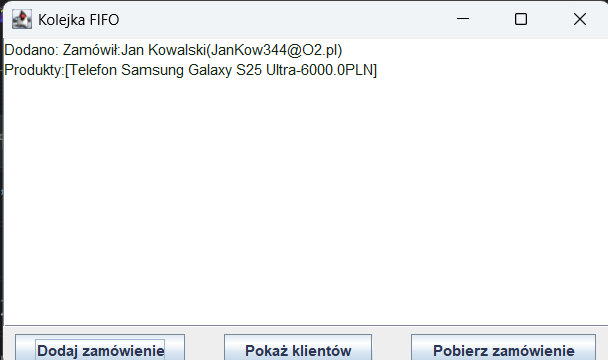
\includegraphics[width=0.7\linewidth]{figures/screenshot007}
	\caption{Wyświetlanie danych dodanego sprzedawcy}
	\label{fig:screenshot007}
\end{figure}


% ------------------------------------------------------------------------
Przetwarzanie zamówień:

Aby przetworzyć zamówienie należy nacisnać przycisk "Pobierz zamówienie". Po przetworzeniu zamówienia
wyświetla się potwierdzenie jego realizacji.
\begin{figure}[H]
	\centering
	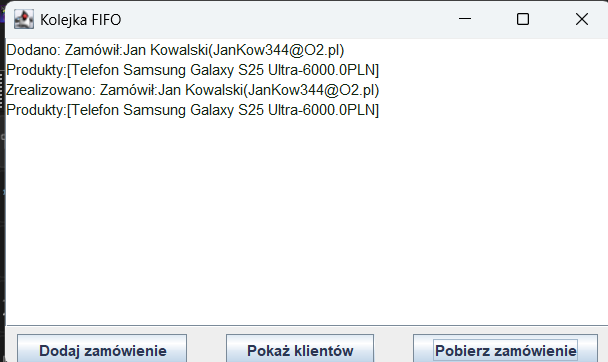
\includegraphics[width=0.7\linewidth]{figures/screenshot008}
	\caption{Realizacja Zamówienia}
	\label{fig:screenshot008}
\end{figure}
W przypadku, próby przetworzenia zamówienia przy pustej kolejce, zostanie wyświetlany napis "Brak
zamówień w kolejce!"
\begin{figure}[H]
	\centering
	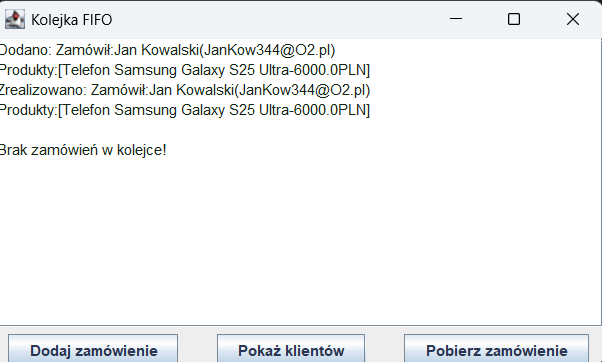
\includegraphics[width=0.7\linewidth]{figures/screenshot009}
	\caption{Próba realizacji zamówienia, gdy kolejka jest pusta}
	\label{fig:screenshot009}
\end{figure}

% ------------------------------------------------------------------------

Naciśnięcie przycisku "pokaż klientów" powoduje wyświetlenie, historii zamówień w bazie danych.
\begin{figure}[H]
	\centering
	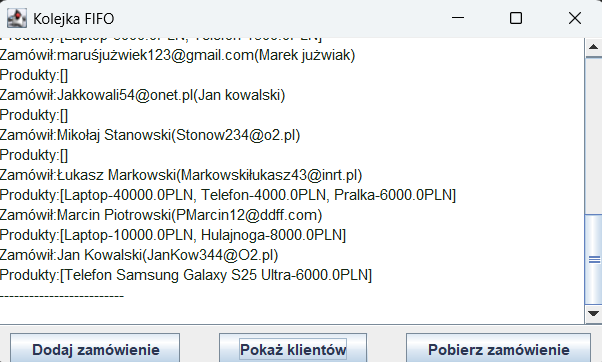
\includegraphics[width=0.7\linewidth]{figures/screenshot010}
	\caption{Wyświetlanie zamówień z bazy danych}
	\label{fig:screenshot010}
\end{figure}


\section{Bazy Danych MySQL}

MySQL to popularny, relacyjny system zarządzania bazami danych, oparty na języku SQL. Jest dostępny jako oprogramowanie open source i rozwijany przez firmę Oracle Corporation. Poniżej znajduje się klasa w języku Java, która odpowiada za połączenie z tą bazą Danych. 
Klasa MenagerBazyDanych:

\lstinputlisting[caption= Klasa MenagerBazyDanych, label=MenagerBazyDanych, style = javaStyle]{src/MenagerBazyDanych.java}


\section{Prezentacja kodu}

Klasa Main (Główna trasa służaca do uruchomienia programu)
\lstinputlisting[style = javaStyle, caption= Klasa Main (główna), label=Main]{src/Main.java}
Klasa GUI (Odpowiedzialna za graficzny interfejs użytkownika)
\lstinputlisting[style = javaStyle, caption= Klasa GUI (Odpowiedzialna za graficzny interfejs użytkownika), label=GUI]{src/GUI.java}
Klasa Klient(Klasa służąca do przechowywania danych klienta)
\lstinputlisting[style = javaStyle, caption= Klasa Klient(Klasa służąca do przechowywania danych klienta), label=Klient]{src/Klient.java}
Klasa Produkt(Klasa służąca do przechowywania informacji o
produkcie)
\lstinputlisting[style = javaStyle, caption= Klasa Produkt(Klasa służąca do przechowywania informacji o produkcie), label=Produkt]{src/Produkt.java}
Klasa Zamówienie
\lstinputlisting[style = javaStyle, caption= Klasa Zamówienia, label=zamowienia]{src/Zamowienie.java}
Klasa KolejkaZamówień
\lstinputlisting[style = javaStyle, caption= Klasa KolejkaZamówień, label=KolejkaZamówień]{src/KolejkaZamowien.java}

% ------------------------------------------------------------------------